\chapter{Introducción}

En el año 2010, se pone en marcha en Montevideo el Sistema de Transporte Metropolitano. El mismo propone el pago de viajes a través de una tarjeta que simplemente se acerca a un dispositivo para efectuarlo. Esa tarjeta logra comunicarse con el dispositivo en forma inalámbrica utilizando radiofrecuencia y se denomina tarjeta RFID. 

\bigskip
El usuario del Sistema de Transporte Metropolitano puede recargar su tarjeta en los puntos de venta. Allí debe presentar su tarjeta e indicar el monto que desea acreditar, un operador recibe la tarjeta y la apoya sobre un dispositivo  que se encuentra conectado a un PC de escritorio. Luego que la tarjeta es leída aparecen en pantalla los datos asociados a la misma, nombre del usuario, saldo disponible, etc., que están almacenados en un servidor centralizado en la Intendencia de Montevideo (IM). El operador utiliza un programa que por un lado registra la transacción en el servidor central de la IM y por otro actualiza el saldo en la tarjeta RFID.

\bigskip
Por razones de seguridad cada  dispositivo de consulta/recarga posee una tarjeta de contactos denominada SAM (Security Access Module) que se utiliza para encriptar las transacciones entre el terminal y el servidor central, y por otro lado se encarga de generar las claves de acceso para la comunicación entre la tarjeta RFID y el terminal.  Esta tarjeta es la encargada de dar seguridad en la transacción de modo que el sistema no sea vulnerable.

\bigskip
Si el usuario desea consultar el saldo disponible en la tarjeta, podrá observarlo en el boleto cuando haga uso de su tarjeta en el ómnibus, o a través de un operador en los puntos de venta.

\bigskip
Se puede desprender de lo anterior, que para poder consultar y/o recargar una tarjeta, es necesario un sistema (ver figura \ref{HW_gral}) que pueda comunicarse con el servidor central de la IM, con las tarjetas RFID de los usuarios a efectos de leerlas y escribirlas, con la tarjeta de seguridad, SAM, y que cuente con algún tipo de interfaz de usuario. 

\begin{figure}[H]
\centering
  \begin{center}
  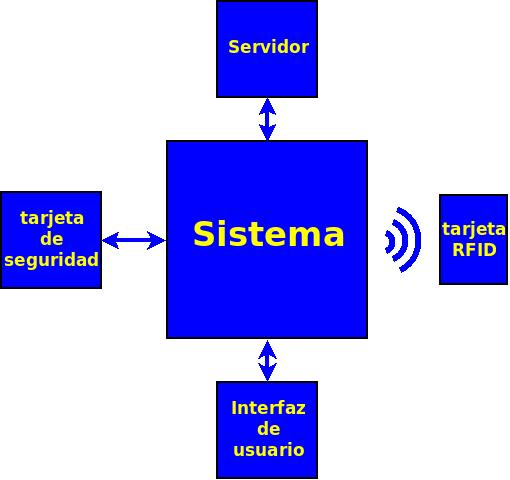
\includegraphics[scale=.4]{Imagenes/diagrama_def.jpg} 
  \end{center}
  \caption{Bloques que conforman el sistema a diseñar}\label{HW_gral} 
\end{figure}

Este proyecto busca desarrollar un dispositivo autónomo, de bajo costo y mantenimiento, que permita realizar estas operaciones funcionando en línea con un servidor, de forma rápida, segura y autogestionada por parte del usuario, sin necesidad de personal, en diversos puntos de Montevideo. 

\bigskip
La propuesta entonces es realizar un dispositivo, a partir del cual se puedan consultar y recargar tarjetas como las utilizadas en el Sistema de Transporte Metropolitano. En este sistema, el usuario que desee consultar el saldo actual no tiene más que acercar su tarjeta y esperar a que el sistema le indique el saldo disponible en la misma. Para poder acreditar saldo en su tarjeta debería antes efectuar el pago de dinero que desea acreditarle, a través de una red de pagos, mensajes de texto, web, o un mecanismo similar que se encuentra desacoplado del sistema implementado. La transacción anterior actualiza el servidor central con el saldo pendiente para que al acercar la tarjeta al dispositivo simplemente se acredite el saldo por el cual se pagó.


\section{Objetivo general}

El objetivo del proyecto es la fabricación de un prototipo de sistema embebido capaz de consultar y recargar tarjetas. Para ésto, como se mencionó en el punto 1.1, deberá lograr establecer comunicación con tarjetas  como las utilizadas en el Sistema de Transporte Metropolitano (comunicación RFID a 13,56 MHz), con tarjetas de contacto (módulo de seguridad SAM), con el usuario a través de una interfaz simple y con el servidor central.

\bigskip
Esto implica entonces la fabricación de dos lectores/escritores de tarjetas, uno para tarjetas RFID (sin contacto) y otro para tarjetas con contacto (SAM), una interfaz para el usuario capaz de informar el estado de la transacción mediante mensajes adecuados, y la utilización de un sistema basado en un microprocesador para controlar los periféricos y realizar las operaciones. Esto último implica además el desarrollo del software para que todo funcione adecuadamente.


\section{Antecedentes}

Existen antecedentes de todas las partes a diseñar.

\bigskip
El lector/escritor de tarjetas empleado en el Sistema de Transporte Metropolitano (IntegriSys iMFR) cumple la función de lectura y escritura de las tarjetas sin contacto y además contiene dentro un lector de tarjetas de contacto usado para la seguridad en las transacciones. Otro ejemplo de lector/escritor de ambos tipos de tarjetas,  es el SCM SDI010.

\bigskip
Hay lectores/escritores exclusivamente de tarjetas de contacto como puede ser el Omnikey 3121, y lectores/escritores de tarjetas sin contacto como el ACR120.

\bigskip
Algo más completo (a nivel hardware), es un dispositivo lector/escritor RFID llamado OpenPCD \cite{OpenPCD}, de hardware abierto, fabricado en Alemania.

\bigskip
El único prototipo completo que se conoce como antecedente es el realizado por el grupo de electrónica de la IM llamado AFE (Artefacto Feo de Exhibir), que realiza lo mismo que se propone pero con un enfoque de diseño diferente, ya que utiliza \\
lectores/escritores de escritorio como los mencionados antes y no de diseño propio.


\section{Alcance}

Respecto al hardware, se fabricará un lector/escritor RFID (basado en el antecedente OpenPCD), un lector de tarjetas de contacto donde se insertará el módulo de seguridad (SAM), una interfaz de usuario donde se incluirá un display, leds y  un indicador sonoro. Se estudiará la forma de conectar dichos periféricos a un sistema central capaz de controlar todas las funcionalidades.

\bigskip
Respecto al software, se desarrollará todo el software necesario para que el sistema funcione, haciendo lo posible para reutilizar código ya implementado para fines similares y lograr la mayor compatibilidad con lo ya existente.


\section{Especificación funcional}

El prototipo final deberá ser capaz de interactuar con tarjetas RFID a través del \\
lector/escritor RFID, con una tarjeta de contacto SAM (seguridad) y con un servidor. Luego de los controles correspondientes en la tarjeta RFID, comenzará la interacción con el usuario mediante un display, leds e indicador sonoro, que será la interfaz de comunicación con el mismo. El display informará al usuario de las tareas que se estén realizando con mensajes cortos y descriptivos. Los tiempos de recarga y consulta deberán ser menores a un minuto.


\section{Criterios de éxito}

El proyecto será considerado exitoso si se logra construir un dispositivo de sistema embebido capaz de consultar y recargar tarjetas RFID, con tiempos de operación razonablemente cortos.

\section{Confidencialidad}

Por motivos de confidencialidad no está permitido divulgar información relativa al módulo de seguridad SAM. 
En particular, no serán nombrados los comandos APDU utilizados para la comunicación con la tarjeta, así como 
tampoco serán agregados dentro del código de la aplicación final de software. Los pasos de autenticación
con este tipo de tarjeta criptográfica tampoco serán detallados en lo que sigue.
En cuanto a las tarjetas sin contacto, RFID, usadas en la aplicación final, no puede detallarse el formato
empleado por el sistema de transporte, STM, para almacernar los datos en los bloques de memoria de la tarjeta.